\chapter{Ergebnisse}
\section{Bewertung des Netzes}
Nach wenigen Testläufen haben sich sehr schnell die optimalen Einstellungen für das Netzwerk festlegen lassen \tabref{settings}.

\begin{table}[h!]
	\centering	
	%\footnotesize
	\begin{tabular}{c|c|c|c|c|c}
	  \textbf{Verst. Schichten} & \textbf{Neuronen} & \textbf{Alpha} & \textbf{Batchsize} & \textbf{Epochen} & \textbf{Durchläufe} \\ \hline 
	  2 & 25 & 0.02 & 260 & 1 & 30.000 \\ 
	\end{tabular}
	\caption{Initialwerte des neuronalen Netzes}
	\label{settings}
\end{table}

Die Erfolgsquote des Netzwerkes liegt ungefähr im selben Bereich wie die der eingesetzten Frameworks von allen teilgenommen Studentengruppen aus dem Sommersemester 2015 \tabref{result}. 

\begin{table}[h!]
	\centering	
	%\footnotesize
	\begin{tabular}{c|c|c}
	  \textbf{Windows Schriftart} & \textbf{Handschrift alt} & \textbf{Handschrift SS2015} \\ \hline 
	  80\% & 50\% & 14\%  \\ 
	\end{tabular}
	\caption{Erkennungsrate mit unterschiedlichen Schriftsätzen}
	\label{result}
\end{table}

Auffällig bei den Ergebnissen, ist das schlechte Abschneiden des neuronalen Netzes bei den Handschriftproben aus dem aktuellen Sommersemester 2015. Eine detaillierte Betrachtung der Ergebnisse zeigt eine häufige nicht-Erkennung von bestimmten Buchstaben \imgref{histogram}. 

\begin{figure}[h!]
	\begin{center}
	\fbox{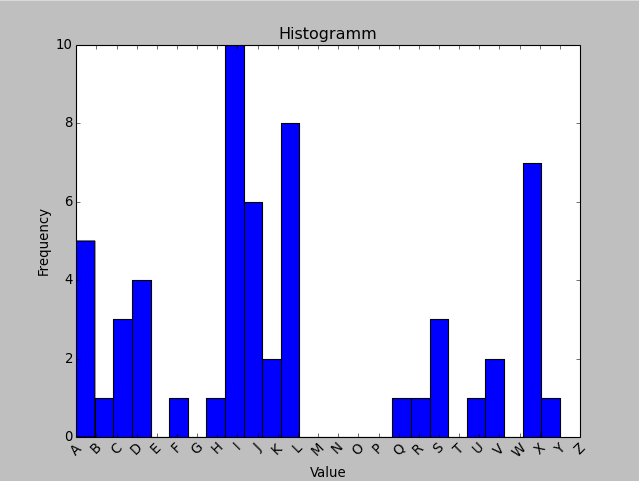
\includegraphics[width=0.8\textwidth]{pictures/histogram.png}}
	\caption{Erkennungsraten}
	\label{histogram}
	\end{center}
\end{figure}

Dieses Ergebnis wurde von den teilnehmenden Gruppen in ihren Auswertungen bestätigt und lässt sich auf mangelhafte Datensätze zurückführen. Beim Vergleich von zuverlässig erkannten und gar nicht erkannten Buchstaben wird die Ursache schnell deutlich \imgref{chars}. Die obersten beiden Zeilen entsprechen Buchstaben aus dem aktuellen Handschriftprobensatz die nicht erkannt wurden. Diese Datensätze sollten im Vorfeld als fehlerhaft aussortiert werden. Die unteren beiden Zeilen stellen hingegen positiv-Beispiele für gute Datensätze dar, die von den neuronalen Netzen in jedem Durchlauf auch zuverlässig erkannt werden können.

\begin{figure}[h!]
	\begin{center}
	\fbox{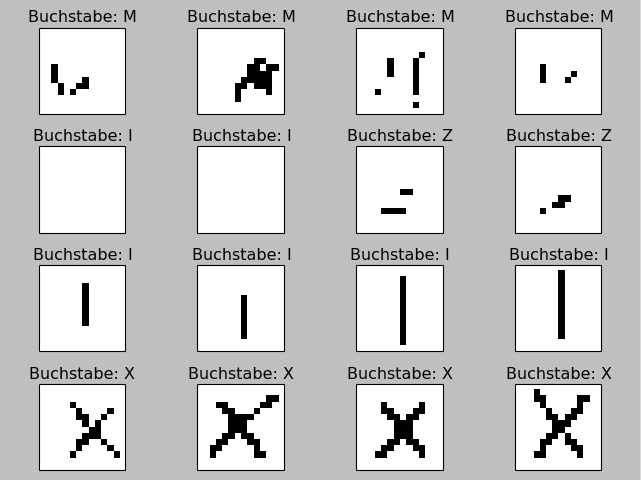
\includegraphics[width=0.6\textwidth]{pictures/chars.png}}
	\caption{Gute und schlechte Handschriftproben}
	\label{chars}
	\end{center}
\end{figure}


\section{Fazit}
Durch die Implementierung eines eigenen neuronalen Netzes konnten die erlernten Grundlagen optimal eingesetzt werden. Das Netzwerk lässt sich durch die gute Übersichtlichkeit, bedingt durch den schlanken Code, schnell anpassen. Änderungen und Erweiterungen lassen sich folglich einfach umsetzen. Im direkten Vergleich zu bestehenden Frameworks ist bei der eigenen Implementierung kein Funktionsoverhead entstanden, wodurch auch die Geschwindigkeit des Netzwerkes profitieren konnte. 

Abschließend lässt sich feststellen, dass sich durch die Konzeption und Implementierung eines eigenen neuronalen Netzes die Anforderungen \chapref{goal} optimal umsetzen ließen. Die Ergebnisse der Handschrifterkennung liegen auf dem selben Niveau der eingesetzten Framworks wie z. B. \emph{PyBrain} \footnote{http://pybrain.org/} von den teilgenommen Studentengruppen. 